\documentclass[a4paper]{article}
\usepackage{student}

% Metadata
\date{\today}
\setmodule{CS110: Computer Architecture}
\setterm{Spring, 2024}

%-------------------------------%
% Other details
%-------------------------------%
\title{Assignment 4: Digital circuit}
\setmembername{Hengyu Ai}  % Fill student name
\setmemberuid{2023533088}  % Fill  student id

%-------------------------------%
% Add / Delete commands and packages
% TODO: Add / Delete here as you need
%-------------------------------%
\usepackage{amsmath,amssymb,bm}
\usepackage{hyperref}
\usepackage{graphicx}
\usepackage{tikz}
\usetikzlibrary{shapes}
\usepackage[utf8]{inputenc}
\usepackage{color}
\usepackage[T1]{fontenc}
\usepackage{color}
\input{glyphtounicode}
\usetikzlibrary{automata} % Import library for drawing automata
\usetikzlibrary{positioning} % ...positioning nodes
\usetikzlibrary{arrows.meta}
\pdfglyphtounicode{visiblespace}{A0}
\pdfglyphtounicode{blank}{A0}
\pdfglyphtounicode{visualspace}{A0}
\pdfglyphtounicode{uni2423}{A0}
\pdfgentounicode=1

\newcommand{\KL}{\mathrm{KL}}
\newcommand{\R}{\mathbb{R}}
\newcommand{\E}{\mathbb{E}}
\newcommand{\T}{\top}

\newcommand{\expdist}[2]{%
        \normalfont{\textsc{Exp}}(#1, #2)%
    }
\newcommand{\expparam}{\bm \lambda}
\newcommand{\Expparam}{\bm \Lambda}
\newcommand{\natparam}{\bm \eta}
\newcommand{\Natparam}{\bm H}
\newcommand{\sufstat}{\bm u}

% Main document
\begin{document}
    % Add header
    \header{}
\textcolor{red}{\textbf{Attention: }}
\textbf{Recommend using \LaTeX \space to complete your work. You can use any tool, such as Logisim, Visio, Draw.io, PowerPoint, etc., to create diagrams. However, handwritten or hand-drawn content is not acceptable.}

\section{Combinational logic}
The circuit shown in Figure.~\ref{fig:Q1_circuit} is a 1-bit comparator. Answer the following questions. \\

\begin{figure}[htbp]
    \centering
    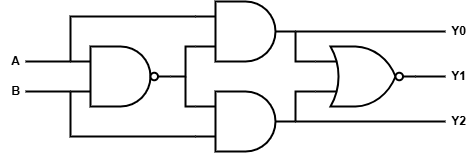
\includegraphics[width=0.8\textwidth]{Q1_circuit.png}
    \caption{A 1-bit comparator circuit}
    \label{fig:Q1_circuit}
\end{figure}

(a) Write the un-simplified logic expressions for $Y0$, $Y1$ and $Y2$. \textbf{[6 pt]}

(b) Draw the truth table of this circuit in the following table.\textbf{[6 pt]}

(c) Write the sum of minterm for $Y0$, $Y1$ and $Y2$. \textbf{[6 pt]}

(d) What comparison do the outputs $Y0$, $Y1$ and $Y2$ represent respectively? e.g: $Y0=1$ represents $A=B$, $A<B$ or $A>B$ (one of the three cases). \textbf{[6 pt]}

(e) Draw the circuit of an unsigned 2-bit comparator using this 1-bit comparator and the following logic gates: 2-input AND, 2-input OR, and 1-input NOT. The 2-bit comparator has two 2-bit inputs $A1A0$ and $B1B0$, three outputs $Y0$, $Y1$ and $Y2$ with the same function as the 1-bit comparator. You can use the 1-bit comparator as a basic logic block as shown in Figure.~\ref{fig:Q1_comparator_1}. \textbf{[10 pt]}

\begin{figure}[htbp]
    \centering
    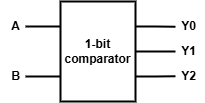
\includegraphics[width=0.4\textwidth]{Q1_comparator_1.png}
    \caption{A 1-bit comparator diagram}
    \label{fig:Q1_comparator_1}
\end{figure}

\newpage

\begin{answer}[Question 1]
    (a)
    \begin{itemize}
        \item \( Y0 = A \overline{AB} \)
        \item \( Y1 = \overline{A \overline{AB} + B \overline{AB}} \)
        \item \( Y2 = B \overline{AB} \)
    \end{itemize}

    (b)
    \begin{center}
        \begin{tabular}{ |c|c||c|c|c| } 
         \hline
         A & B & Y2 & Y1 & Y0 \\ 
         \hline
         0 & 0 & 0 & 1 & 0 \\ 
         \hline
         0 & 1 & 1 & 0 & 0 \\ 
         \hline
         1 & 0 & 0 & 0 & 1 \\
         \hline
         1 & 1 & 0 & 1 & 0 \\
         \hline
        \end{tabular}
    \end{center}

    (c)\\

    Minterms:
    \begin{center}
    \begin{tabular}{c|c}
    \( \overline{AB} \) & \( m_0 \) \\
    \( A \overline{B} \) & \( m_1 \) \\
    \( \overline{A} B \) & \( m_2 \) \\
    \( AB \) & \( m_3 \) \\
    \end{tabular}
    \end{center}

    \begin{itemize}
        \item \( Y0 = m_2 \)
        \item \( Y1 = m_0 + m_3 \)
        \item \( Y2 = m_1 \)
    \end{itemize}

    (d)

    \begin{itemize}
        \item \( Y0 = 1 \) represents  \( A > B \)
        \item \( Y1 = 1 \) represents \( A = B \)
        \item \( Y2 = 1 \) represents \( A < B \)
    \end{itemize}

    \newpage

    (e)\\
    \begin{center}
    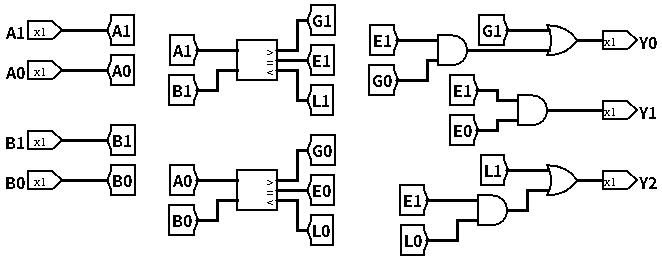
\includegraphics[width=0.8\textwidth]{Q1_d.png}
    \end{center}

\end{answer}

\newpage
\section{SDS}
 In the following circuit, NOT gates have a delay of 1ns, AND gates have a delay of 4ns, NAND gates have a delay of 3ns, OR gates have a delay of 4ns, NOR gates have a delay of 3ns. The registers have a clk-to-q delay of 2ns and setup time of 2ns. Assume the inputs
 come from registers. All the delays refer to propagation delay.\\
 
\begin{figure}[hp]
    \centering
    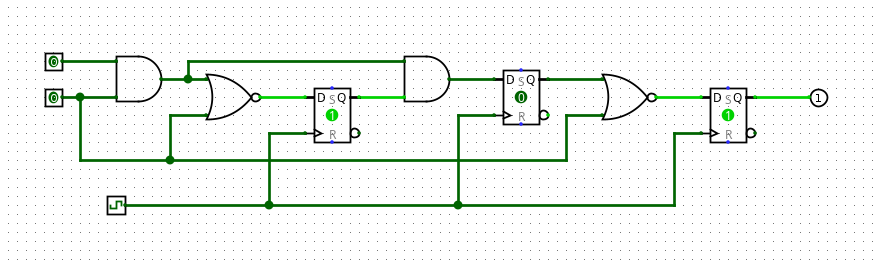
\includegraphics[width=1.0\textwidth]{Q2.png}
    \caption{Circuit Diagram}
    \label{fig:q2}
\end{figure}

What is the minimum acceptable clock cycle time for this circuit? What
 clock frequency does it correspond to? (please include enough explanation) \textbf{[16 pt]}
 
\begin{answer}[Question 2]
    The minimum clock cycle time is determined by the longest path delay in the circuit.
    The longest path from a register to a register is as follows:

    \begin{itemize}
        \item upper input
        \item and gate (4 ns)
        \item and gate (4 ns)
        \item register in the middle
    \end{itemize}

    Therefore:

    \[
    t_{clk} \ge t_{setup} + t_{clk-to-q} + t_{comp} = 2 + 2 + 8 = 12 \text{ ns}
    \]

    The minimum clock cycle time is 12 ns.\\
    The maximum clock frequency is the reciprocal of the clock cycle time:
    \[
    f_{max} = \frac{1}{t_{clk}} = \frac{1}{12 \text{ ns}} = 83.33 \text{ MHz}
    \]
\end{answer}

\newpage
\section{Finite state machine}
In this part, you need to implement a detector. When receiving two or more successive '0's or '1's, it outputs 1. For a bit sequence, it inputs one bit a period from left to right. e.g: input='11101001', output='01100010'.

(a) Draw the FSM (Moore machine) for this detector in five states: \{start\}, \{10\}(discrete '0'), \{01\}(discrete '1'), \{00\}(successive '0's), \{11\}(successive '1's). \\
e.g: input='011001', state=\{start\}$\xrightarrow{}$\{10\}$\xrightarrow{}$\{01\}$\xrightarrow{}$\{11\}$\xrightarrow{}$\{10\}$\xrightarrow{}$\{00\}$\xrightarrow{}$\{01\} \textbf{[10 pt]}

(b) Draw the FSM (Mealy machine) for this detector in no more than three states.\textbf{[10 pt]}

(c) Assign '000' to represent state \{start\}, '110' to represent \{10\}, '101' to represent \{01\}, '100' to represent \{00\}, '111' to represent \{11\}. We use 'CS' to represent current state and 'NS' for next state. Fill the truth table for the next-state and output logic based on the Moore FSM. \textbf{[15 pt]}

(d) Draw the circuit diagram for NS and output. \textbf{[15 pt]}
\begin{answer}[Question 3]
    (a)
    \begin{center}
    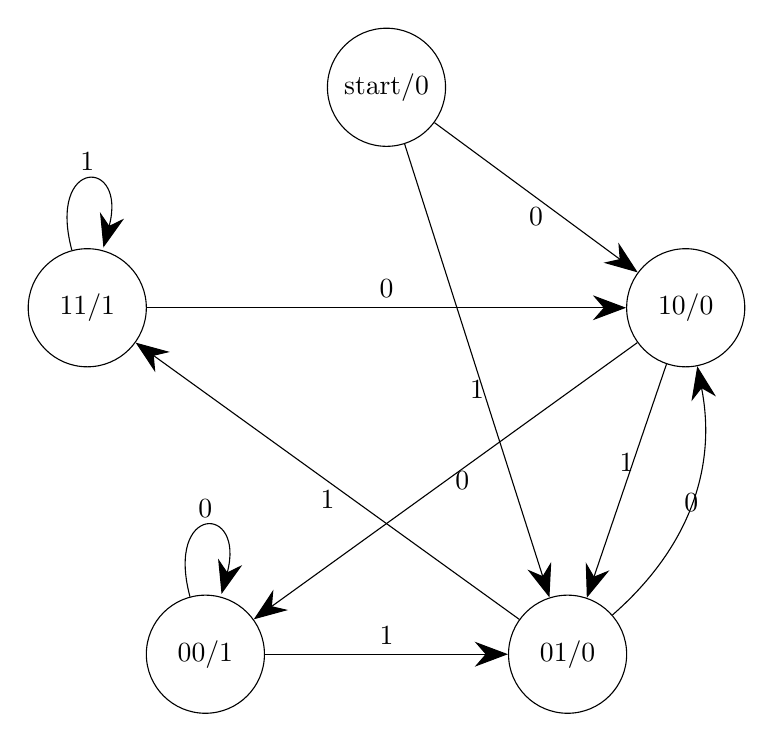
\begin{tikzpicture}[->, >={Stealth[scale=2.5]}]
        \node[state, minimum size=15mm] (s1) at (0,4) {start/0};  
        \node[state, minimum size=15mm] (s2) at (3.8,1.2) {10/0};  
        \node[state, minimum size=15mm] (s3) at (2.3,-3.2) {01/0};
        \node[state, minimum size=15mm] (s4) at (-2.3,-3.2) {00/1};
        \node[state, minimum size=15mm] (s5) at (-3.8,1.2) {11/1};
        
        \draw (s1) edge [below] node {0} (s2);
        \draw (s1) edge [below] node {1} (s3);
        \draw (s2) edge [right] node {0} (s4);
        \draw (s2) edge [above] node {1} (s3);
        \draw (s3) edge [bend right] node {0} (s2);
        \draw (s3) edge [below] node {1} (s5);
        \draw (s4) edge [loop above] node {0} (s4);
        \draw (s4) edge [above] node {1} (s3);
        \draw (s5) edge [loop above] node {1} (s5);
        \draw (s5) edge [above] node {0} (s2);
    \end{tikzpicture}
    \end{center}

    \newpage
    (b)
    \begin{center}
    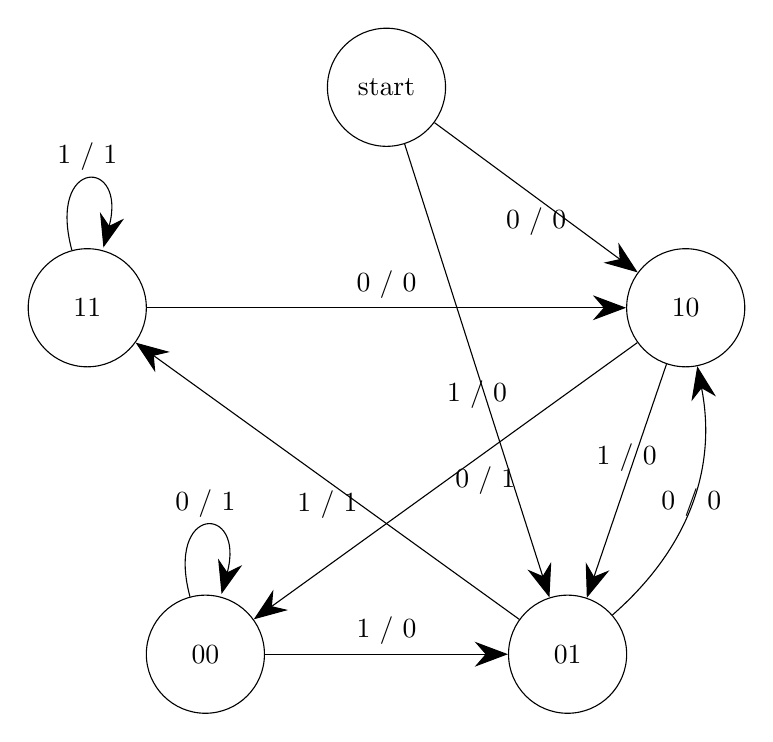
\begin{tikzpicture}[->, >={Stealth[scale=2.5]}]
        \node[state, minimum size=15mm] (s1) at (0,4) {start};  
        \node[state, minimum size=15mm] (s2) at (3.8,1.2) {10};  
        \node[state, minimum size=15mm] (s3) at (2.3,-3.2) {01};
        \node[state, minimum size=15mm] (s4) at (-2.3,-3.2) {00};
        \node[state, minimum size=15mm] (s5) at (-3.8,1.2) {11};
        
        \draw (s1) edge [below] node {0 / 0} (s2);
        \draw (s1) edge [below] node {1 / 0} (s3);
        \draw (s2) edge [right] node {0 / 1} (s4);
        \draw (s2) edge [above] node {1 / 0} (s3);
        \draw (s3) edge [bend right] node {0 / 0} (s2);
        \draw (s3) edge [below] node {1 / 1} (s5);
        \draw (s4) edge [loop above] node {0 / 1} (s4);
        \draw (s4) edge [above] node {1 / 0} (s3);
        \draw (s5) edge [loop above] node {1 / 1} (s5);
        \draw (s5) edge [above] node {0 / 0} (s2);
    \end{tikzpicture}
    \end{center}

    (c) Do not modify the given values in the truth table.\\
    \begin{center}
        \begin{tabular}{ |c|c|c|c||c|c|c|c| } 
            \hline
            CS[2] & CS[1] & CS[0] & input & NS[2] & NS[1] & NS[0] & output \\ 
            \hline
            0 & 0 & 0 & 0 & 1 & 1 & 0 & 0 \\ 
            \hline
            0 & 0 & 0 & 1 & 1 & 0 & 1 & 0 \\ 
            \hline
            1 & 1 & 0 & 0 & 1 & 0 & 0 & 1 \\ 
            \hline
            1 & 1 & 0 & 1 & 1 & 0 & 1 & 0 \\ 
            \hline
            1 & 0 & 1 & 0 & 1 & 1 & 0 & 0 \\ 
            \hline
            1 & 0 & 1 & 1 & 1 & 1 & 1 & 1 \\ 
            \hline
            1 & 0 & 0 & 0 & 1 & 0 & 0 & 1 \\ 
            \hline
            1 & 0 & 0 & 1 & 1 & 0 & 1 & 0 \\ 
            \hline
            1 & 1 & 1 & 0 & 1 & 1 & 0 & 0 \\ 
            \hline
            1 & 1 & 1 & 1 & 1 & 1 & 1 & 1 \\ 
            \hline
        \end{tabular}
    \end{center}

    (d)

    Main circuit:
    \begin{center}
        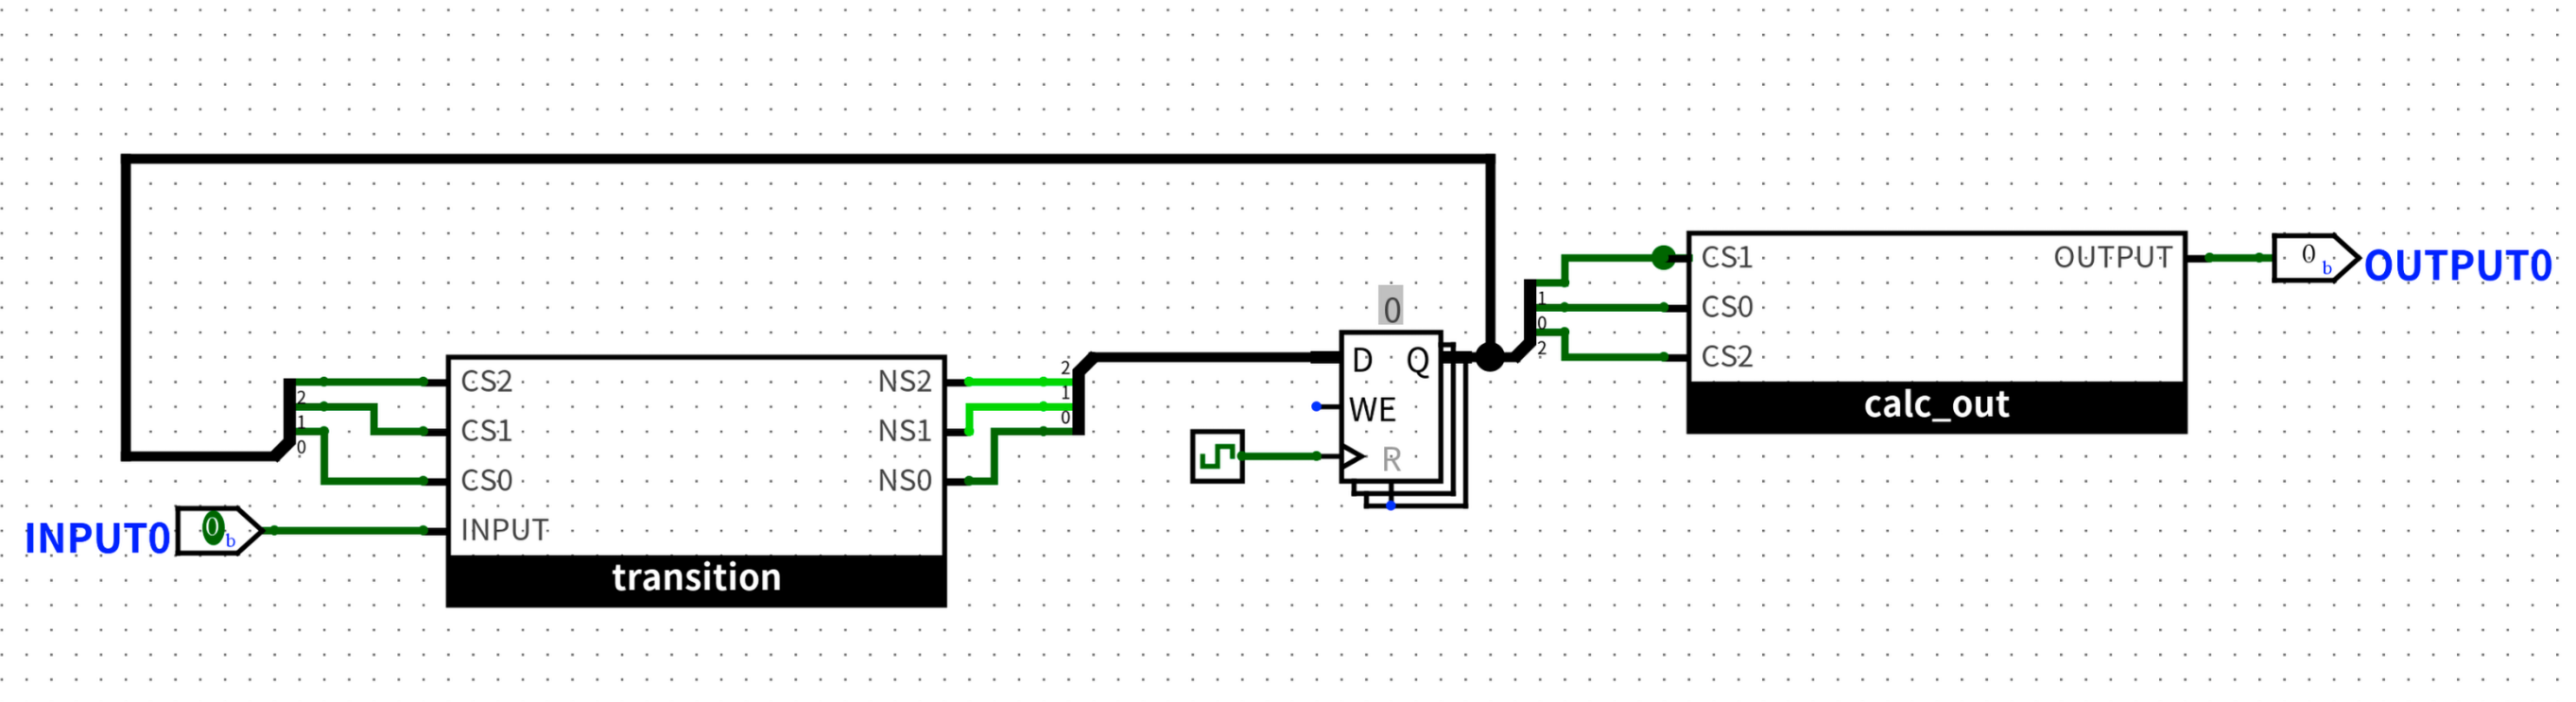
\includegraphics[width=0.9\textwidth]{main.png}
    \end{center}

    \newpage

    Transition circuit:
    \begin{center}
        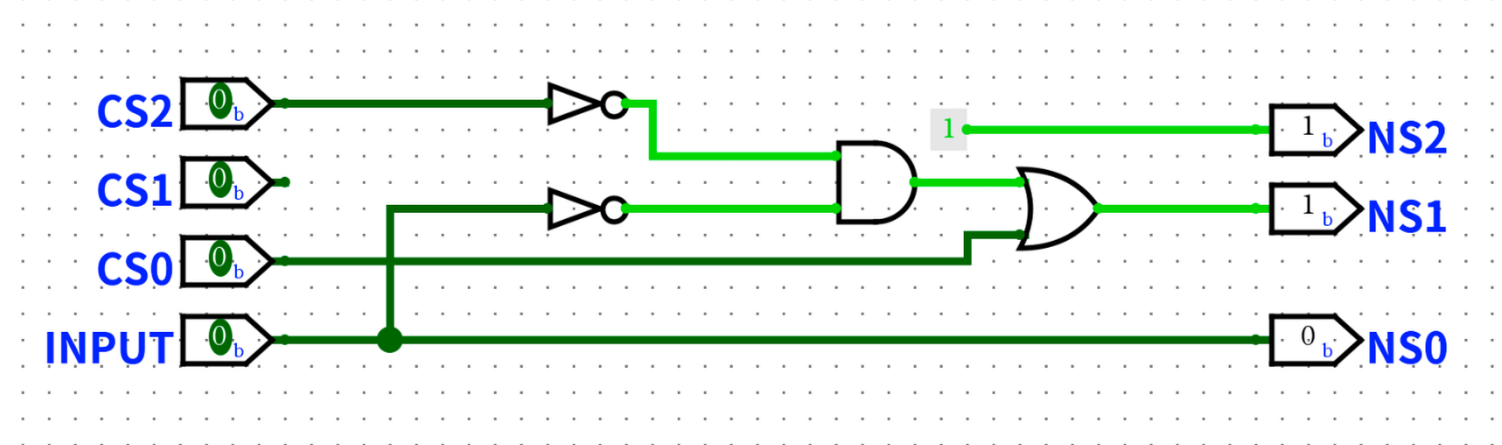
\includegraphics[width=0.9\textwidth]{transition.png}
    \end{center}

    Output circuit:
    \begin{center}
        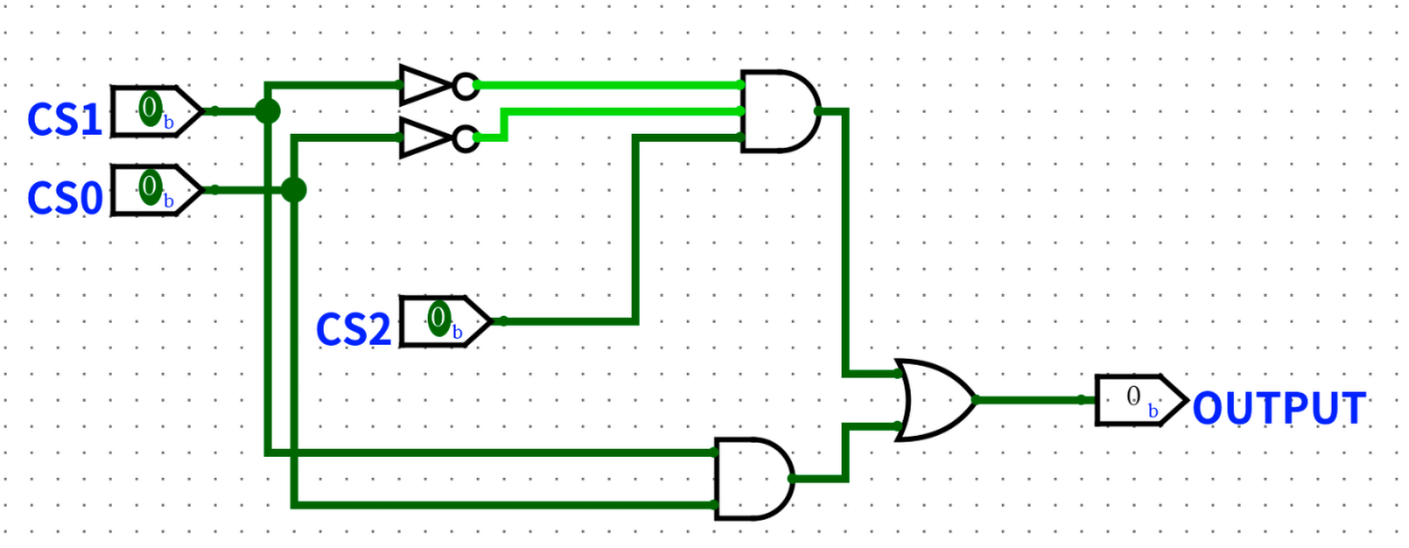
\includegraphics[width=0.9\textwidth]{calc_out.png}
    \end{center}
        
\end{answer}

\end{document}
